%
\section{Experiments}
\label{sec:experiments}


To train our model, which we label as \textit{ITW}, we use a variant of the Basel Face Model (BFM)~\cite{paysan20093d} that we trained to contain both identities drawn from the original BFM model along with expressions provided by~\cite{cao2014facewarehouse}. 
We trained the ``in-the-wild'' texture model on the images of iBUG, LFPW \& AFW datasets~\cite{sagonas2016faces} as described in Sec.~\ref{sec:texture-model} using the 3D shape fits provided by~\cite{Zhu_2016_CVPR}. Additionally, we elect to use the project-out formulation for the throughout our experiments due its superior run-time performance and equivalent fitting performance to the simultaneous one.


\subsection{3D Shape Recovery}
\label{sec:experiments-quantitative-shape}
Herein, we evaluate our ``in-the-wild'' 3DMM (\textit{ITW}) in terms of 3D shape estimation accuracy against two popular state-of-the-art alternative 3DMM formulations. The first one is a classic 3DMM with the original Basel laboratory texture model and full lighting equation which we term
\textit{Classic}. The second is the texture-less linear model proposed in~\cite{huber2015fitting,huber2016multiresolution} which we refer to as~\textit{Linear}. For \textit{Linear} code we use the Surrey Model with related blendshapes along with the implementation given in~\cite{huber2016multiresolution}. 

\begin{figure}[!t]
    \centering
    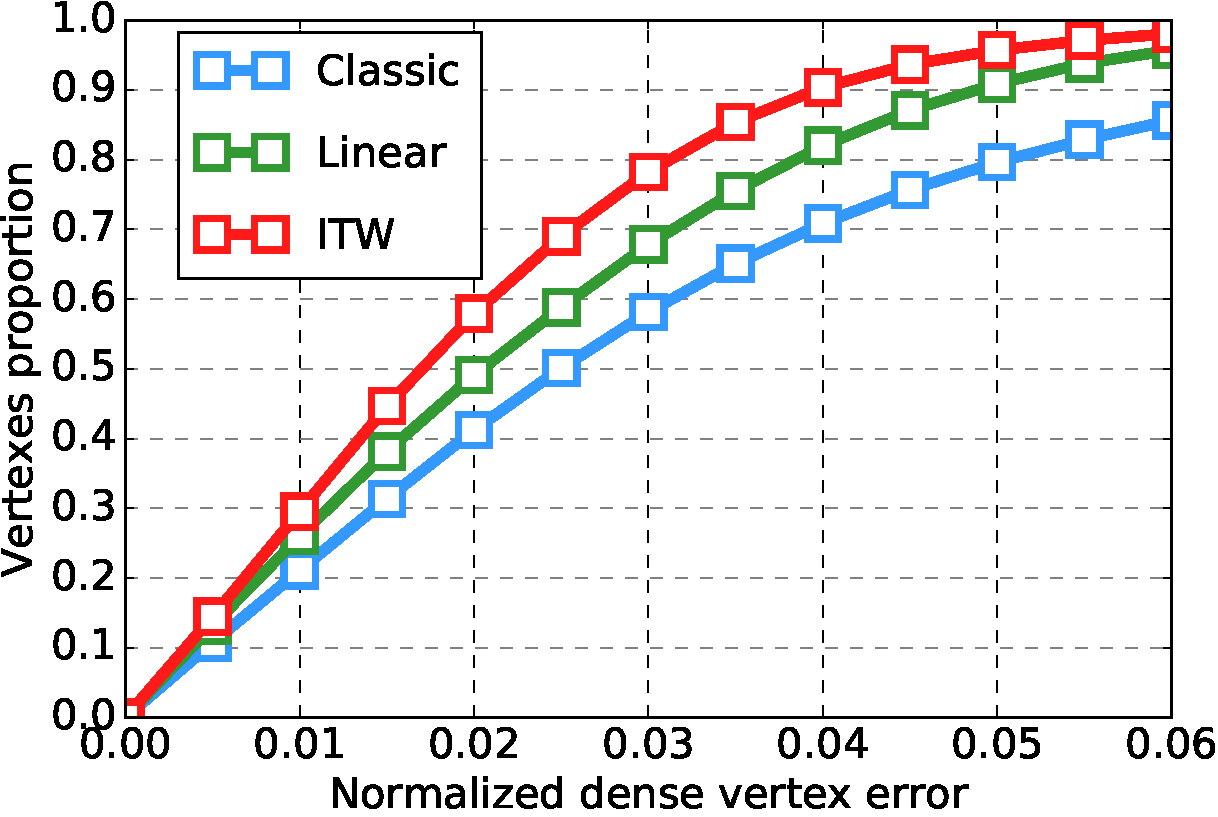
\includegraphics[width=\linewidth]{exp_3dmm}
    \caption{Accuracy results for facial shape estimation on KF-ITW database. The 
    results are presented as Cumulative Error Distributions of the normalized dense vertex error. Table~\ref{tab:kf_dense_fit_error_ced} reports additional measures.}
    \label{fig:kf_dense_fit_error_ced}
\end{figure}

We use the ground-truth annotations provided in the KF-ITW dataset to initialize and fit all three techniques to the ``in-the-wild'' style images in the dataset. The mean mesh of each model under test is landmarked with the same 49-point markup used in the dataset, and is registered against the ground truth mesh by performing a Procrustes alignment using the sparse annotations followed by Non-Rigid Iterative Closest Point (N-ICP) to iteratively deform the two surfaces until they are brought into correspondence.
This provides a per-model `ground-truth' for the 3D shape recovery problem for each image under test.
Our error metric is the per-vertex dense error between the recovered shape and the model-specific corresponded ground-truth fit, normalized by the inter-ocular distance for the test mesh.
Fig.~\ref{fig:kf_dense_fit_error_ced} shows the cumulative error distribution for this experiment for the three models under test. Table~\ref{tab:kf_dense_fit_error_ced} reports the corresponding Area Under the Curve (AUC) and failure rates. The \emph{Classic} model
struggles to fit to the ``in-the-wild'' conditions present in the test set, and performs the worst.
The texture-free \textit{Linear} model does better, but the \textit{ITW} model is most able to recover the facial shapes due to its ideal feature basis for the ``in-the-wild'' conditions.

Figure~\ref{fig:example_gallery} demonstrates qualitative results on a wide range of fits of ``in-the-wild'' images drawn from the Helen and 300W datasets~\cite{sagonas2016faces,sagonas2013300} that qualitatively highlight the effectiveness of the proposed technique.
We note that in a wide variety of expression, identity, lighting and occlusion conditions our model is able to robustly reconstruct a realistic 3D facial shape that stands up to scrutiny.

\begin{table}[!t]
\centering
\begin{tabular}{|l|cc|}
\hline
\emph{Method} & \emph{AUC} & \emph{Failure Rate (\%)} \\
\hline\hline
\textbf{ITW}     & \textbf{0.678} & \textbf{1.79} \\
Linear  & 0.615 & 4.02 \\
Classic & 0.531 & 13.9 \\
\hline
\end{tabular}
\caption{Accuracy results for facial shape estimation on KF-ITW database. The 
    table reports the Area Under the Curve (AUC) and Failure Rate of the Cumulative Error Distributions of Fig.~\ref{fig:kf_dense_fit_error_ced}.}
\label{tab:kf_dense_fit_error_ced}
\end{table}


\begin{figure}[!t]
    \centering
    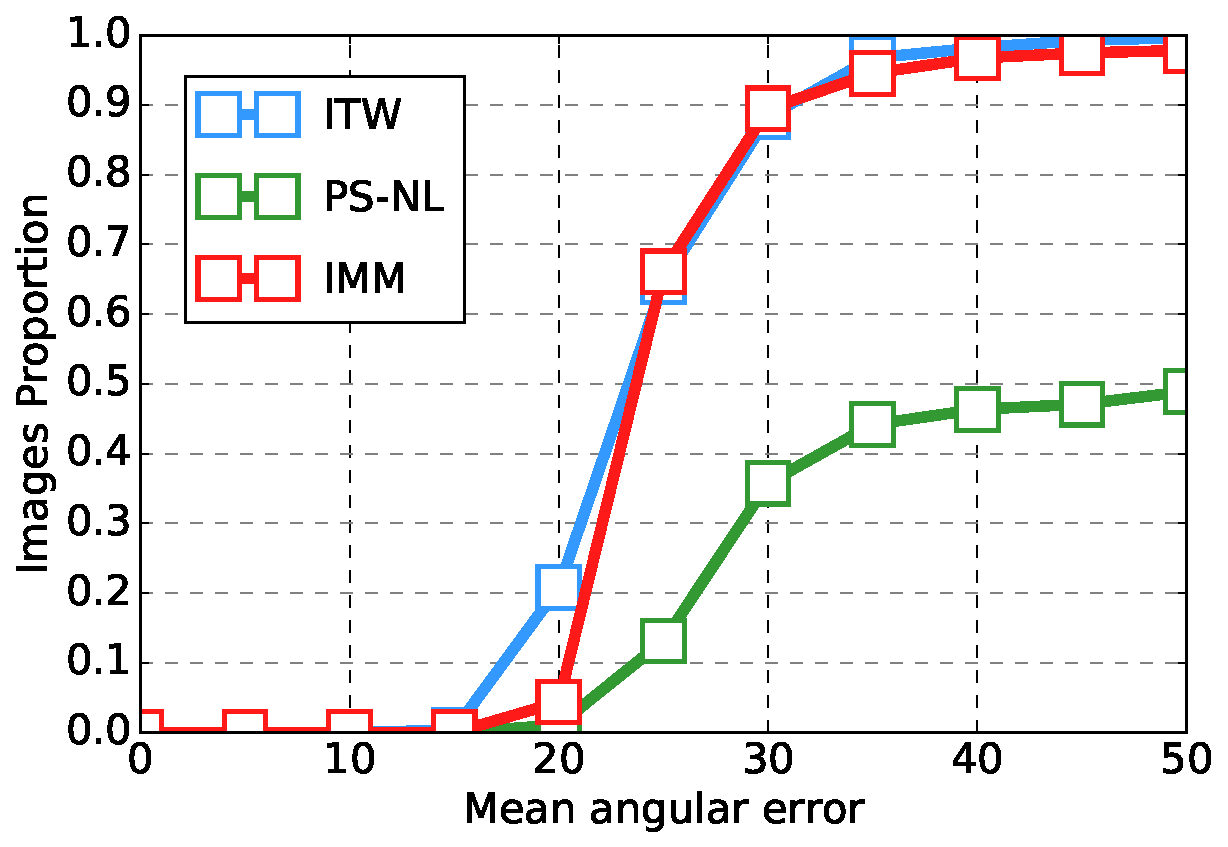
\includegraphics[width=\linewidth]{photoface_mms}
    \caption{Results on facial surface normal estimation in the form of Cumulative Error Distribution of mean angular error.}
\label{fig:angular_normals_ced}
\end{figure}


\begin{figure*}
\centering
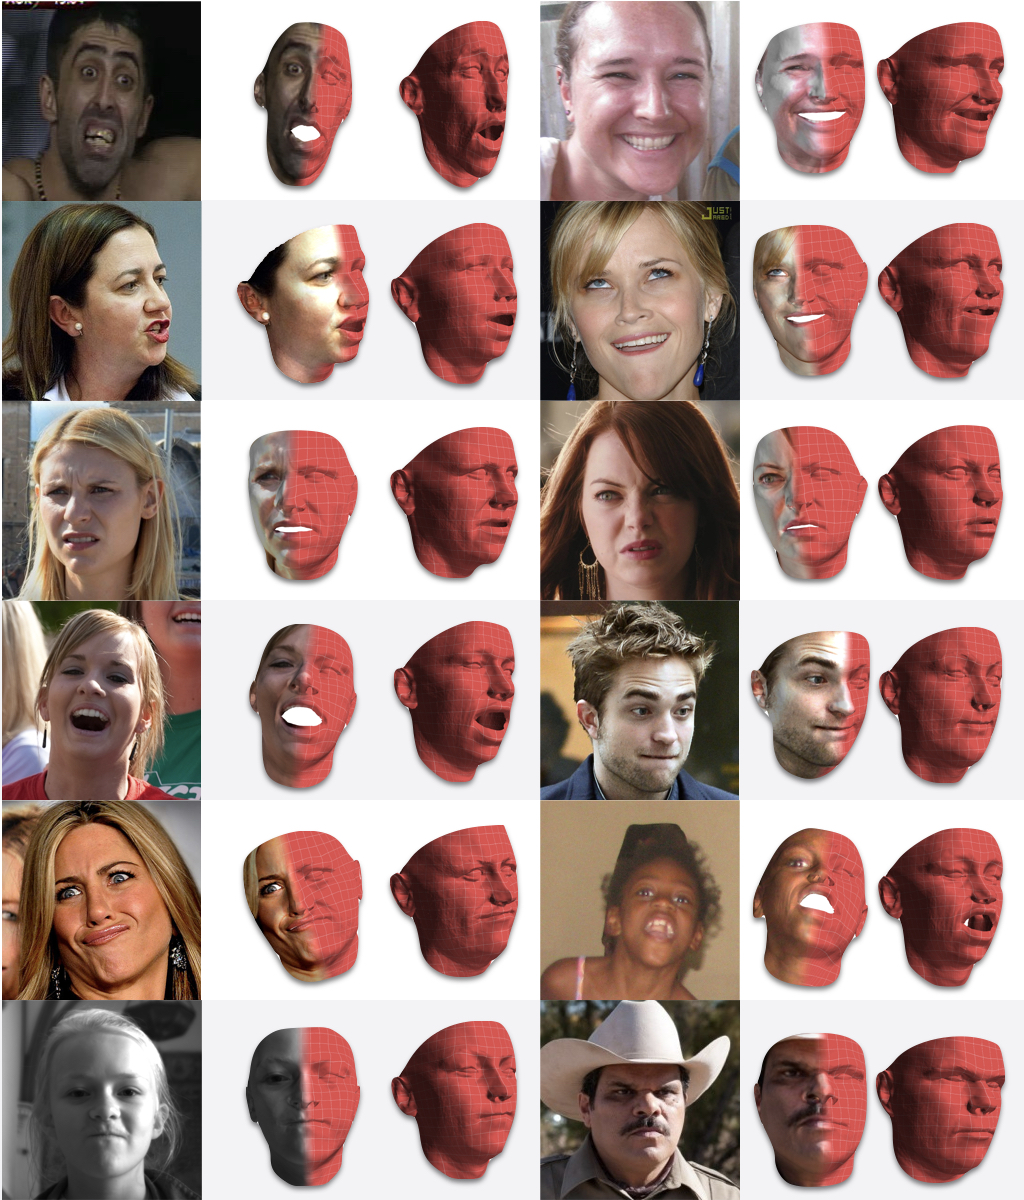
\includegraphics[width=0.95\linewidth]{example_gallery}
\caption{Examples of in the wild fits of our \emph{ITW} 3DMM taken from 300W~\cite{sagonas2016faces}.}
\label{fig:example_gallery}
\end{figure*}


\subsection{Quantitative Normal Recovery}
\label{sec:experiments-quantitative-normals}
As a second evaluation, we use our technique to find per-pixel normals and compare against two well established Shape-from-Shading~(SfS) techniques:~\textit{PS-NL}~\cite{basri2007photometric} and \textit{IMM}~\cite{kemelmacher2013internet}. For experimental evaluation we employ images of 100 subjects from the Photoface database~\cite{photoface}. As a set of four illumination conditions are provided for each subject then we can generate ground-truth facial surface normals using calibrated 4-source Photometric Stereo~\cite{marr1978representation}. In~Fig.~\ref{fig:angular_normals_ced} we show the cumulative error distribution in terms of the mean angular error. \textit{ITW} slightly outperforms \textit{IMM} even though both \textit{IMM} and \textit{PS-NL} use all four available images of each subject.

%

%


%
%
%
%
%
%
%
%
%
